\documentclass{beamer}

%%%%%%%%%%%%%%%%%%%%%%%%%%%%%%%%%%%%
%%     Include packages          %%
%%%%%%%%%%%%%%%%%%%%%%%%%%%%%%%%%%%%
\usepackage[utf8]{inputenc} % Allows using UTF-8

\usepackage[a4paper, margin=2.56cm]{geometry} % Set-up page and margins

% To insert the pdf frontpage
\usepackage{pdfpages}

% Including some maths utilities
\usepackage{amsmath}
\usepackage{amsfonts}
\usepackage{amsthm}
\usepackage{amssymb}
\DeclareMathOperator*{\argmax}{arg\,max}
\DeclareMathOperator*{\argmin}{arg\,min}


%
% the environments 'definition', 'lemma', 'proposition', 'corollary',
% 'remark', and 'example' are defined in the LLNCS documentclass as well.
%
\newtheorem{definition}{Definition}
\newtheorem{theorem}{Theorem}
\newtheorem{lemma}{Lemma}
\newtheorem{proposition}{Proposition}
\newtheorem{corollary}{Corollary}
\newtheorem{remark}{Remark}
\newtheorem{example}{Example}


% Fancy space between paragraphs
\usepackage{parskip}
\setlength{\parindent}{0em}
\setlength{\parskip}{1em}

% Automatic Month, Year in title
\usepackage{datetime}
\newdateformat{monthyeardate}{
  \monthname[\THEMONTH], \THEYEAR}

% Fancy packages to write pseudocode
\usepackage{algorithm}
\usepackage{algpseudocode}

% Package to import source code and format it
\usepackage{listings}

% Produce more beautiful tables
\usepackage{booktabs}

% Nice hyperlinks inside document
\usepackage[hidelinks]{hyperref}

% Allows enumerating
\usepackage{enumerate}% http://ctan.org/pkg/enumerate

% Required to insert images
\usepackage{graphicx} 

\usepackage[
	citestyle=ieee, 
    bibstyle=ieee,
    style=numeric-comp,
    sorting=nty,
    maxbibnames=99, % Make sure we are printing all authors in the appendix
    backend=biber
]{biblatex}

% Needed to add subcaptions to subfigures
\usepackage{caption}
\usepackage{subcaption}

% Allows using foreach
\usepackage{pgffor}

% Avoids placing floats before section
\usepackage[section]{placeins} 

% Allow to have content in multiple columns
\usepackage{multicol}

% Cool diagrams
\usepackage{tikz}
\usetikzlibrary{positioning,quotes,shapes.geometric,arrows.meta}
\pgfdeclarelayer{nodelayer} 
\pgfdeclarelayer{edgelayer}
\pgfdeclarelayer{embeded}
\pgfdeclarelayer{stages}
\pgfsetlayers{main,nodelayer,edgelayer,stages,embeded}
\tikzstyle{new style 0}=[fill=white, draw=black, shape=circle, align=center]
\tikzstyle{tree_edge}=[-, draw=black]
\tikzstyle{opChan}=[-Stealth, black]
\tikzstyle{daChan}=[-Stealth, red]
\tikzstyle{io}=[trapezium, trapezium angle=67, trapezium stretches body, fill=blue!30, draw=black, thick]
\tikzstyle {filter_gen} = [rectangle, rounded corners, text centered, draw=black, fill=blue!30, thick]
\tikzset{
  invisible/.style={opacity=0},
  visible on/.style={alt={#1{}{invisible}}},
  alt/.code args={<#1>#2#3}{%
    \alt<#1>{\pgfkeysalso{#2}}{\pgfkeysalso{#3}} % \pgfkeysalso doesn't change the path
  },
}
\usepackage{pgf}

% Protect caption to allow \verb
\usepackage{cprotect}
%%%%%%%%%%%%%%%%%%%%%%%%%%%%%%%%%%%%
%%        Usefull macros          %%
%%%%%%%%%%%%%%%%%%%%%%%%%%%%%%%%%%%%

\newcommand{\mst}{\texorpdfstring{$\mathsf{MST}$}{MST}}
\newcommand{\msts}{\texorpdfstring{$\mathsf{MST}s$}{MSTs}}
\newcommand{\mstof}[1]{$\mathsf{MST}_{#1}$}
\newcommand{\dynmst}{\mathsf{Dynamic\_MST}}
\newcommand{\dpm}{\texorpdfstring{$\mathsf{DPA}$}{DPA}}
\newcommand{\DP}{$\mathsf{DP}$}
%\newcommand{\DPmst}{\texorpdfstring{$\mathsf{DP_{MST}}$}{DP\_MST}}
%\newcommand{\DPmstv}[1]{$\mathsf{DP_{MST\_{#1}}}$}

\newcommand{\DPmst}{\texttt{DP\_{Kruskal}}}
\newcommand{\DPmstv}[1]{\texttt{DP\_{Kruskal\_{#1}}}}

\newcommand{\FKruskal}{\texttt{Filter\_{Kruskal}}}
\newcommand{\Kruskal}{\texttt{Kruskal}}

\newcommand{\opinsert}[0]{{\tt insert}}
\newcommand{\opupdate}[0]{{\tt update}}
\newcommand{\opremove}[0]{{\tt remove}}
\newcommand{\opmst}[0]{{\tt mst}}

\newcommand{\Go}{{\tt Go}}
\newcommand{\Golang}{{\tt Golang}}

\newcommand{\AD}[1]{{\color{red} AD: #1} \PackageWarning{teaching}{Comment from AD}}
\newcommand{\DB}[1]{{\color{blue} DB: #1}\PackageWarning{teaching}{Comment from DB}}
\newcommand{\EP}[1]{{\color{magenta} EP: #1}\PackageWarning{teaching}{Comment from EP}}


%%%%%%%%%%%%%%%%%%%%%%%%%%%%%%%%%%%%
%%        Other setups            %%
%%%%%%%%%%%%%%%%%%%%%%%%%%%%%%%%%%%%

\addbibresource{references.bib} % Adds the bibliography

\title{TFM-DanielBenedí}
\author{Daniel Benedí}
\date{\monthyeardate}



%------------------------------------------------------------
%This block of code defines the information to appear in the
%Title page
\title[Dyn. MST on Dynamic Pipeline] %optional
{Maintaining the Minimum Spanning Forest of Fully Dynamic Graphs on the Dynamic Pipeline Approach}

\author[D. Benedí] % (optional)
{Daniel Benedí}

\institute[UPC] % (optional)
{
  Facultat d'Informàtica de Barcelona\\
  Universitat Politècnica de Catalunya
}

\date[\monthyeardate\today] % (optional)
{\monthyeardate\today}

\logo{\includegraphics[height=0.75cm]{UPC.png}}


%End of title page configuration block

\begin{document}

%The next statement creates the title page.
\frame{\titlepage}

\begin{frame}{Overview}
    \tableofcontents
\end{frame}


%---------------------------------------------------------




%---------------------------------------------------------
%Changing visivility of the text

\section{Preliminaries}

\begin{frame}{Preliminaries: Dynamic Graphs}
\begin{columns}
    \column{0.4\textwidth}
    \centering
    \uncover<4->{At the beginning:}\\
    \resizebox{\textwidth}{!}{%
        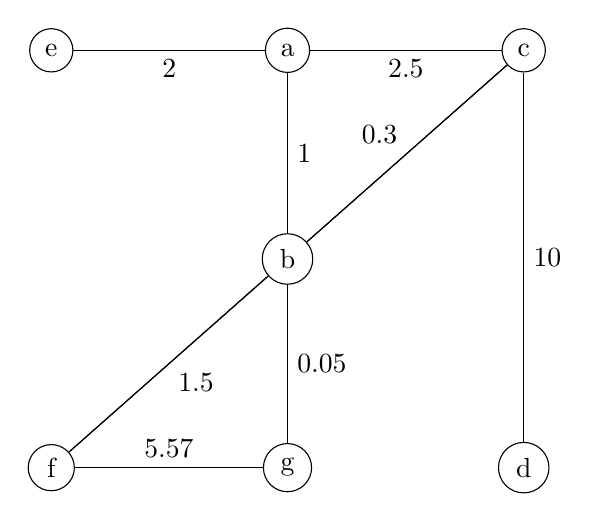
\begin{tikzpicture}
            \begin{pgfonlayer}{nodelayer}
                \node [style=new style 0, visible on=<1->] (0) at (-4, 2.65) {a};
                \node [style=new style 0, visible on=<1->] (1) at (-4, 0) {b};
                \node [style=new style 0, visible on=<1->] (2) at (-1, 2.65) {c};
                \node [style=new style 0, visible on=<1->] (3) at (-1, -2.65) {d};
                \node [style=new style 0, visible on=<1->] (4) at (-7, 2.65) {e};
                \node [style=new style 0, visible on=<1->] (5) at (-7, -2.65) {f};
                \node [style=new style 0, visible on=<1->] (6) at (-4, -2.65) {g};
            \end{pgfonlayer}
            \begin{pgfonlayer}{edgelayer}
                \draw [style={tree_edge}, visible on=<2>] (0) to (1);
                \draw [style={tree_edge}, visible on=<2>] (1) to (2);
                \draw [style={tree_edge}, visible on=<2>] (2) to (0);
                \draw [style={tree_edge}, visible on=<2>] (2) to (3);
                \draw [style={tree_edge}, visible on=<2>] (0) to (4);
                \draw [style={tree_edge}, visible on=<2>] (1) to (5);
                \draw [style={tree_edge}, visible on=<2>] (5) to (6);
                \draw [style={tree_edge}, visible on=<2>] (1) to (6);
                \draw [style={tree_edge}, visible on=<3->] (0) to["1"] (1);
                \draw [style={tree_edge}, visible on=<3->] (1) to["0.3"] (2);
                \draw [style={tree_edge}, visible on=<3->] (2) to["2.5"] (0);
                \draw [style={tree_edge}, visible on=<3->] (2) to["10"] (3);
                \draw [style={tree_edge}, visible on=<3->] (0) to["2"] (4);
                \draw [style={tree_edge}, visible on=<3->] (1) to["1.5"] (5);
                \draw [style={tree_edge}, visible on=<3->] (5) to["5.57"] (6);
                \draw [style={tree_edge}, visible on=<3->] (1) to["0.05"] (6);
            \end{pgfonlayer}
        \end{tikzpicture}
    }
    \column{0.3\textwidth}
    
    \scalebox{0.8}{\begin{minipage}{1.20\textwidth}
        \begin{itemize}
            \item<4-> Initial Graph
            \item<5-> \alt<5>{\textcolor{blue}{\texttt{INSERT,b,e,0.08}}}{\texttt{INSERT,b,e,0.08}}
            \item<5-> \alt<5>{\textcolor{blue}{\texttt{INSERT,a,d,5}}}{\texttt{INSERT,a,d,5}}
            \item<5-> \alt<5>{\textcolor{blue}{\texttt{INSERT,d,g,2.6}}}{\texttt{INSERT,d,g,2.6}}
            \item<5-> \alt<5>{\textcolor{red}{\texttt{DELETE,a,b}}}{\texttt{DELETE,a,b}}
            \item<6-> \alt<6>{\textcolor{red}{\texttt{DELETE,c,d}}}{\texttt{DELETE,c,d}}
            \item<6-> \alt<6>{\textcolor{blue}{\texttt{INSERT,a,b,1}}}{\texttt{INSERT,a,b,1}}
            \item<7-> \alt<7>{\textcolor{magenta}{\texttt{UPDATE,f,g,4.42}}}{\texttt{UPDATE,f,g,4.42}}
            \item<7-> \alt<7>{\textcolor{magenta}{\texttt{UPDATE,b,e,2.85}}}{\texttt{UPDATE,b,e,2.85}}
        \end{itemize}
    \end{minipage}}
    \column{0.4\textwidth}
    \centering
    \visible<4->{With the operations:}
    \resizebox{\textwidth}{!}{%
        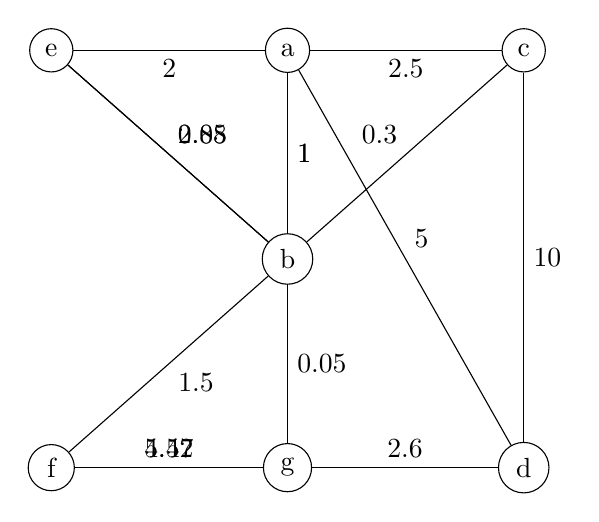
\begin{tikzpicture}
            \begin{pgfonlayer}{nodelayer}
                \node [style=new style 0, visible on=<4->] (0) at (-4, 2.65) {a};
                \node [style=new style 0, visible on=<4->] (1) at (-4, 0) {b};
                \node [style=new style 0, visible on=<4->] (2) at (-1, 2.65) {c};
                \node [style=new style 0, visible on=<4->] (3) at (-1, -2.65) {d};
                \node [style=new style 0, visible on=<4->] (4) at (-7, 2.65) {e};
                \node [style=new style 0, visible on=<4->] (5) at (-7, -2.65) {f};
                \node [style=new style 0, visible on=<4->] (6) at (-4, -2.65) {g};
            \end{pgfonlayer}
            \begin{pgfonlayer}{edgelayer}
                \draw [style={tree_edge},visible on=<4-5>,alt=<5>{red, dashed}{black}] (0) to["1"] (1);
                \draw [style={tree_edge},visible on=<6->,alt=<6>{blue}{black}] (0) to["1"] (1);
                \draw [style={tree_edge}, visible on=<4->] (1) to["0.3"] (2);
                \draw [style={tree_edge}, visible on=<4->] (2) to["2.5"] (0);
                \draw [style={tree_edge},visible on=<4-6>,alt=<6>{red, dashed}{black}] (2) to["10"] (3);
                \draw [style={tree_edge}, visible on=<4->] (0) to["2"] (4);
                \draw [style={tree_edge}, visible on=<4->] (1) to["1.5"] (5);
                \draw [style={tree_edge},visible on=<4-6>] (5) to["5.57"] (6);
                \draw [style={tree_edge},visible on=<7->, alt=<7>{magenta}{black}] (5) to["4.42"] (6);
                \draw [style={tree_edge}, visible on=<4->] (1) to["0.05"] (6);
                \draw [style={tree_edge},visible on=<5-6>,alt=<5>{blue}{black}] (4) to["0.08"] (1);
                \draw [style={tree_edge},visible on=<7->,alt=<7>{magenta}{black}] (4) to["2.85"] (1);
                \draw [style={tree_edge},visible on=<5->,alt=<5>{blue}{black}] (0) to["5"] (3);
                \draw [style={tree_edge},visible on=<5->,alt=<5>{blue}{black}] (6) to["2.6"] (3);
            \end{pgfonlayer}
        \end{tikzpicture}
    }
\end{columns}
\end{frame}

\begin{frame}{Preliminaries: Minimum Spanning Forest}
    \begin{definition}
        A \emph{spanning tree $T$ of a graph $G$} is a subgraph that is a tree and includes all the vertices of $G$.
    \end{definition}
    
    \begin{figure}[!h]
        \centering
        \begin{subfigure}{0.48\linewidth}
            \scalebox{0.75}{
                \tikzstyle{new style 0}=[fill=white, draw=black, shape=circle, align=center]
\tikzstyle{tree_edge}=[-, draw=black]

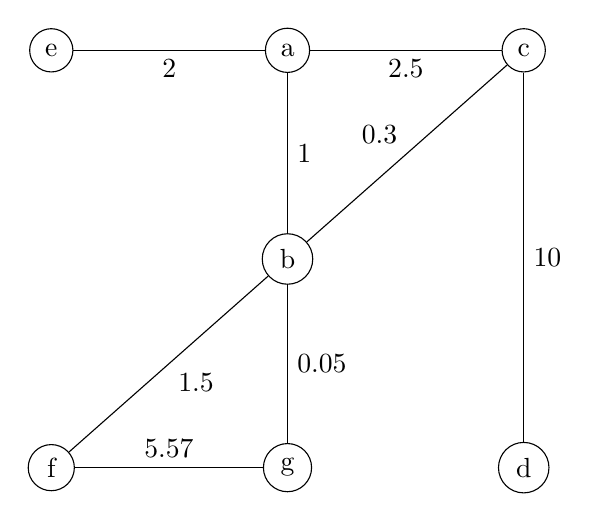
\begin{tikzpicture}
	\begin{pgfonlayer}{nodelayer}
		\node [style=new style 0] (0) at (-4, 2.65) {a};
		\node [style=new style 0] (1) at (-4, 0) {b};
		\node [style=new style 0] (2) at (-1, 2.65) {c};
		\node [style=new style 0] (3) at (-1, -2.65) {d};
		\node [style=new style 0] (4) at (-7, 2.65) {e};
		\node [style=new style 0] (5) at (-7, -2.65) {f};
		\node [style=new style 0] (6) at (-4, -2.65) {g};
	\end{pgfonlayer}
	\begin{pgfonlayer}{edgelayer}
		\draw [style={tree_edge}] (0) to["1"] (1);
		\draw [style={tree_edge}] (1) to["0.3"] (2);
		\draw [style={tree_edge}] (2) to["2.5"] (0);
		\draw [style={tree_edge}] (2) to["10"] (3);
		\draw [style={tree_edge}] (0) to["2"] (4);
		\draw [style={tree_edge}] (1) to["1.5"] (5);
		\draw [style={tree_edge}] (5) to["5.57"] (6);
		\draw [style={tree_edge}] (1) to["0.05"] (6);
	\end{pgfonlayer}
\end{tikzpicture}
            }
        \end{subfigure}
        \begin{subfigure}{0.48\linewidth}
            \scalebox{0.75}{
                \input{figures/spanning_example.tikz}
            }
        \end{subfigure}
    \end{figure}
\end{frame}

\begin{frame}{Preliminaries: Motivation} \justifying
    There are many theoretical and experimental results. Cattaneo et al. (2002) showed that simpler algorithm are faster in practice than those with better asymptotically behaviour. Those results used small graphs due to limitations of the date.
    
    \textcolor{white}{Here goes some text}
    
    Almost no algorithms for maintaining dynamic \msts\ on concurrent or parallel set-ups. Up to our knowledge, only one with batch updates in MapReduce.
\end{frame}

\section{Graphs and \msts\ in \dpm}
\begin{frame}{Graphs and \msts\ in \dpm: Underlying forest and \mst\ (I)}
    \begin{definition}\label{def:u-forest}
        Given a graph $G=(V,E)$, we say that the sequence $F_G = \langle T_1,\dots,T_k\rangle$, $k \ge 1$, 
        is an \emph{underlying forest} of $G$ 
        if $T_i \subseteq E$ $\forall i$, $\cup_{i=1}^k T_i = E$, $\forall i,j, i\neq j, T_i\cap T_j = \emptyset$
        and  $\forall i\:\: T_i\in F_G$ there exists a distinguished vertex $v_i\in V$, called the \emph{root} 
        of $T_i$, such that $\forall e \in T_i$,  $e$ is incident to $v_i$.
    \end{definition}

    \textcolor{white}{Here goes some text}
    
    \resizebox{\textwidth}{!}{
    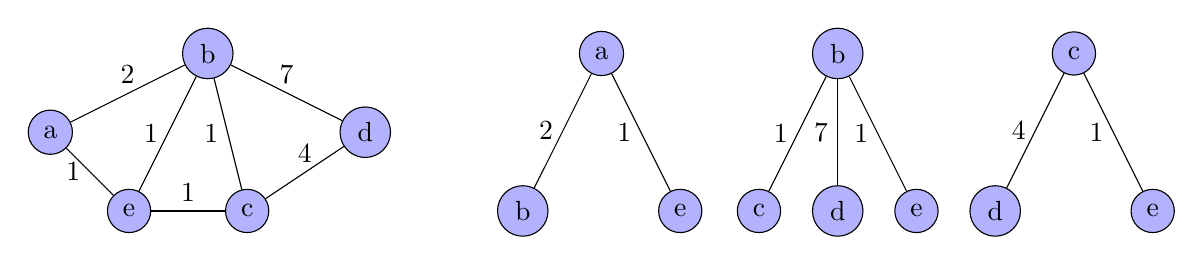
\begin{tikzpicture}
        \node[shape=circle,draw=black, fill = blue!30] (a) at (-3,0) {a};
        \node[shape=circle,draw=black, fill = blue!30] (b) at (-1,1) {b};
        \node[shape=circle,draw=black, fill = blue!30] (c) at (-0.5,-1) {c};
        \node[shape=circle,draw=black, fill = blue!30] (d) at (1,0) {d};
        \node[shape=circle,draw=black, fill = blue!30] (e) at (-2,-1) {e};
    
        \path [-] (a) edge node[above] {$2$} (b);
        \path [-](a) edge node[left] {$1$} (e);
        \path [-](b) edge node[left] {$1$} (e);
        \path [-](b) edge node[left] {$1$} (c);
        \path [-](b) edge node[above] {$7$} (d);
        \path [-](c) edge node[above] {$4$} (d);
        \path [-](e) edge node[above] {$1$} (c);  
    
        \node[shape=circle,draw=black, fill = blue!30] (f) at (4,1) {a};
        \node[shape=circle,draw=black, fill = blue!30] (g) at (3,-1) {b};
        \node[shape=circle,draw=black, fill = blue!30] (h) at (5,-1) {e};
      
        \path [-] (f) edge node[left] {$2$} (g);
        \path [-](f) edge node[left] {$1$} (h);
    
        \node[shape=circle,draw=black, fill = blue!30] (i) at (7,1) {b};
        \node[shape=circle,draw=black, fill = blue!30] (j) at (6,-1) {c};
        \node[shape=circle,draw=black, fill = blue!30] (k) at (7,-1) {d};
        \node[shape=circle,draw=black, fill = blue!30] (l) at (8,-1) {e};
      
        \path [-] (i) edge node[left] {$1$} (j);
        \path [-](i) edge node[left] {$7$} (k);
        \path [-](i) edge node[left] {$1$} (l);
    
        \node[shape=circle,draw=black, fill = blue!30] (m) at (10,1) {c};
        \node[shape=circle,draw=black, fill = blue!30] (n) at (9,-1) {d};
        \node[shape=circle,draw=black, fill = blue!30] (o) at (11,-1) {e};
      
        \path [-] (m) edge node[left] {$4$} (n);
        \path [-](m) edge node[left] {$1$} (o);
    \end{tikzpicture}
    }
\end{frame}

\begin{frame}{Graphs and \msts\ in \dpm: Underlying forest and \mst\ (II)}
        \begin{proposition}
        Given a weighted graph $G=(V,E)$ represented by the underlying forest 
        $F_G = \langle T_1, \dots, T_k\rangle\ (k \ge 1)$ and the subgraphs $G_i$, $1\leq i\leq k$, of $G$ 
        such that $G_i = \cup_{j=1}^kT_i$, it holds that
            \[
                \mathsf{MST}(G_i) =     \left\{ \begin{array}{lr}
        				                    T_1& \mbox{if}\:\: i = 1 \\ 
        				                    \mathsf{MST}(T_i \cup \mathsf{MST}(G_{i-1})) & \mbox{if}\:\: i > 1 \\
        			                \end{array}\right.
            \]
        where \mst(G) is any correct procedure to compute a \mst\ of $G$.
    \end{proposition}
\end{frame}

\begin{frame}{Graphs and \msts\ in \dpm: Stages of Dynamic Pipeline}
    \begin{itemize}
        \item<2-> \textbf{Source:} This stage manages the in-connection with the outside: streaming input, file reading, random generation...
        \item<3-> \textbf{Sink:} This stage manages the out-connection. Usually stdout
        \item<4-> \textbf{Generator:} If operation requires to be processed by a filter, it will generate a new filter.
        \item<5-> \textbf{Filter:} This (statefull) stage will select which operations to perform and wich ones have to be passed to the next filter. It will do the main work.
    \end{itemize}
    
    \centering
    \begin{tikzpicture}
        \begin{pgfonlayer}{nodelayer}
            \node [style=io, minimum height=1.25cm, minimum width=3.5cm, shape border rotate=270, visible on=<2->] (0) at (-3, 0) {Source};
            \node [style=filter_gen, minimum width=1cm, minimum height=2.5cm, visible on=<5->] (1) at (-1, 0) {Filter};
            \node [style=filter_gen, minimum width=1cm, minimum height=2.5cm, visible on=<5->] (2) at (0.9, 0) {Filter};
            \node [style=filter_gen, minimum width=1cm, minimum height=2.5cm, align=center, visible on=<4->] (3) at (3.2, 0) {Generator \\ \includegraphics[width=.05\textwidth]{gear} };
            \node [style=io, minimum height=1.25cm, minimum width=3.5cm, shape border rotate=90, visible on=<3->] (4) at (5.7, 0) {Sink};
        \end{pgfonlayer}
        \begin{pgfonlayer}{edgelayer}
            \draw [style={opChan}, visible on=<6->] ([yshift=0.5 cm]0.east) to["Op"] ([yshift=0.5 cm]1.west);
            \draw [style={opChan}, visible on=<6->] ([yshift=0.5 cm]1.east) to["Op"] ([yshift=0.5 cm]2.west);
            \draw [style={opChan}, visible on=<6->] ([yshift=0.5 cm]2.east) to["Op"] ([yshift=0.5 cm]3.west);
            \draw [style={opChan}, visible on=<6->] ([yshift=0.5 cm]3.east) to["Op"] ([yshift=0.5 cm]4.west);
            
            \draw [style={daChan}, visible on=<6->] ([yshift=-0.5 cm]0.east) to["Data"] ([yshift=-0.5 cm]1.west);
            \draw [style={daChan}, visible on=<6->] ([yshift=-0.5 cm]1.east) to["Data"] ([yshift=-0.5 cm]2.west);
            \draw [style={daChan, visible on=<6->}] ([yshift=-0.5 cm]2.east) to["Data"] ([yshift=-0.5 cm]3.west);
            \draw [style={daChan}, visible on=<6->] ([yshift=-0.5 cm]3.east) to["Data"] ([yshift=-0.5 cm]4.west);
        \end{pgfonlayer}
    \end{tikzpicture}
\end{frame}

\begin{frame}{Graphs and \msts\ in \dpm: \DPmst}
    \begin{center}
    \resizebox{1\textwidth}{!}{
    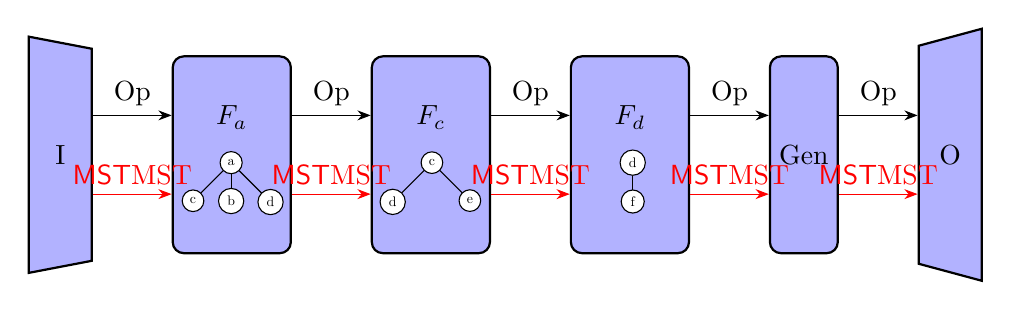
\begin{tikzpicture}
        \begin{pgfonlayer}{nodelayer}
            \node [style=io, minimum height=0.8cm, minimum width=3cm, shape border rotate=270] (In) at (0, 0) {I};
            \node [style=filter_gen, minimum width=1.5cm, minimum height=2.5cm, right= 1cm of In,  text depth = 1cm] (F1) {$F_a$};
            \node [style=filter_gen, minimum width=1.5cm, minimum height=2.5cm, right= 1cm of F1,  text depth = 1cm] (F2) {$F_c$};
            \node [style=filter_gen, minimum width=1.5cm, minimum height=2.5cm, right= 1cm of F2,  text depth = 1cm] (F3) {$F_d$};
            \node [style=filter_gen, minimum width=0.8cm, minimum height=2.5cm, align=center, right= 1cm of F3] (Gen) {Gen};
            \node [style=io, minimum height=0.8cm, minimum width=3.2cm, shape border rotate=90, right= 1cm of Gen] (Out) {O};
        \end{pgfonlayer}
        \begin{pgfonlayer}{edgelayer}
                \draw [style={opChan}] ([yshift=0.5 cm]Gen.east) to["Op"] ([yshift=0.5 cm]Out.west);
                \draw [style={daChan}] ([yshift=-0.5 cm]Gen.east) to["\mst\ "] ([yshift=-0.5 cm]Out.west);

                \draw [style={opChan}] ([yshift=0.5 cm]In.east) to["Op"] ([yshift=0.5 cm]F1.west);
                \draw [style={daChan}] ([yshift=-0.5 cm]In.east) to["\mst\ "] ([yshift=-0.5 cm]F1.west);
                
                \draw [style={opChan}] ([yshift=0.5 cm]F1.east) to["Op"] ([yshift=0.5 cm]F2.west);
                \draw [style={daChan}] ([yshift=-0.5 cm]F1.east) to["\mst\ "] ([yshift=-0.5 cm]F2.west);
                
                \draw [style={opChan}] ([yshift=0.5 cm]F2.east) to["Op"] ([yshift=0.5 cm]F3.west);
                \draw [style={daChan}] ([yshift=-0.5 cm]F2.east) to["\mst\ "] ([yshift=-0.5 cm]F3.west);
                \draw [style={opChan}] ([yshift=0.5 cm]F3.east) to["Op"] ([yshift=0.5 cm]Gen.west);
                \draw [style={daChan}] ([yshift=-0.5 cm]F3.east) to["\mst\ "] ([yshift=-0.5 cm]Gen.west);
        \end{pgfonlayer}

        \begin{pgfonlayer}{embeded}
            %Filter 1
            \node [style=new style 0, scale=0.5] (a1) at (2.17, -0.1) {a};
            \node [style=new style 0, scale=0.5,below=0.18cm of a1] (b1) {b};
            \node [style=new style 0, scale=0.5,below left=0.4cm of a1] (c1) {c};
            \node [style=new style 0, scale=0.5,below right=0.4cm of a1] (d1) {d};
            \draw[style={tree_edge}]{} (a1) to (b1);
            \draw[style={tree_edge}]{} (a1) to (c1);
            \draw[style={tree_edge}]{} (a1) to (d1);
            
            %Filter 2
            \node [style=new style 0, scale=0.5] (c2) at (4.72, -0.1) {c};
            \node [style=new style 0, scale=0.5,below left=0.4cm of c2] (d2) {d};
            \node [style=new style 0, scale=0.5,below right=0.4cm of c2] (e2) {e};
            \draw[style={tree_edge}]{} (c2) to (d2);
            \draw[style={tree_edge}]{} (c2) to (e2);
            
            %Filter 3
            \node [style=new style 0, scale=0.5] (d3) at (7.27, -0.1) {d};
            \node [style=new style 0, scale=0.5,below=0.18cm of d3] (f3) {f};
            \draw[style={tree_edge}]{} (d3) to (f3);
        \end{pgfonlayer}
    \end{tikzpicture}
    }
    \end{center}

    \resizebox{0.9\textwidth}{!}{
    %Input MST
    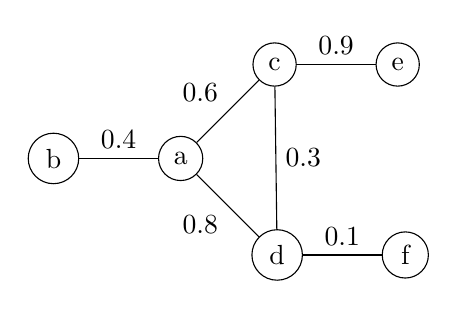
\begin{tikzpicture}
        \begin{pgfonlayer}{nodelayer}
            \node[style=new style 0] (a) at (0,0) {a};
            \node[style=new style 0, left=1cm of a] (b) {b};
            \node[style=new style 0, above right=1.118cm of a] (c) {c};
            \node[style=new style 0, below right=1.118cm of a] (d) {d};
            \node[style=new style 0, right=1cm of c] (e) {e};
            \node[style=new style 0, right=1cm of d] (f) {f};
        \end{pgfonlayer}
        \begin{pgfonlayer}{edgelayer}
            \draw[style={tree_edge}]{} (b) to["0.4"] (a);
            \draw[style={tree_edge}]{} (c) to["0.3"] (d);
            \draw[style={tree_edge}]{} (a) to["0.6"] (c);
            \draw[style={tree_edge}]{} (d) to["0.1"] (f);
            \draw[style={tree_edge}]{} (d) to["0.8"] (a);
            \draw[style={tree_edge}]{} (c) to["0.9"] (e);
        \end{pgfonlayer}
    \end{tikzpicture}
    
    %Output MST
    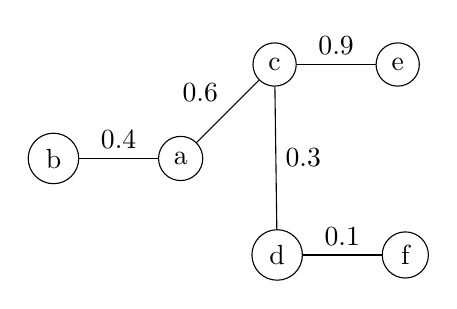
\begin{tikzpicture}
        \begin{pgfonlayer}{nodelayer}
            \node[style=new style 0] (a) at (0,0) {a};
            \node[style=new style 0, left=1cm of a] (b) {b};
            \node[style=new style 0, above right=1.118cm of a] (c) {c};
            \node[style=new style 0, below right=1.118cm of a] (d) {d};
            \node[style=new style 0, right=1cm of c] (e) {e};
            \node[style=new style 0, right=1cm of d] (f) {f};
        \end{pgfonlayer}
        \begin{pgfonlayer}{edgelayer}
            \draw[style={tree_edge}]{} (b) to["0.4"] (a);
            \draw[style={tree_edge}]{} (c) to["0.3"] (d);
            \draw[style={tree_edge}]{} (a) to["0.6"] (c);
            \draw[style={tree_edge}]{} (d) to["0.1"] (f);
            \draw[style={tree_edge}]{} (c) to["0.9"] (e);
        \end{pgfonlayer}
    \end{tikzpicture}
    }    
    
\end{frame}


\begin{frame}{Graphs and \msts\ in \dpm: \DPmst}
            \centering
            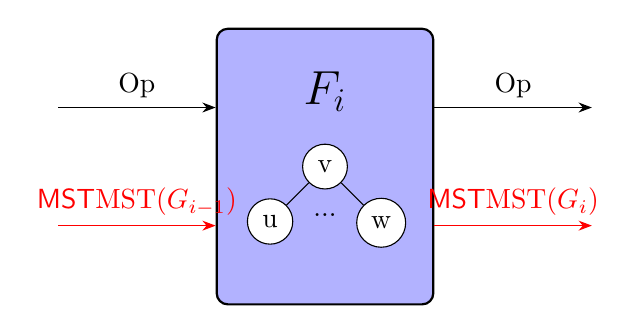
\begin{tikzpicture}                
                \node [style=filter_gen, minimum width=2.75cm, minimum height=3.5cm,  text depth = 2cm] (Fi) at (0.0, 0.0) {\LARGE $F_i$};

                \node [ left=2cm of Fi] (prev) {};
                \node [right=2cm of Fi] (post) {};

                % Input channels
                \draw [style={opChan}] ([yshift=0.75 cm]prev.east) to["Op"] ([yshift=0.75 cm]Fi.west);
                \draw [style={daChan}] ([yshift=-0.75 cm]prev.east) to["\mst($G_{i-1}$)"] ([yshift=-0.75 cm]Fi.west);

                % Output channels
                \draw [style={opChan}] ([yshift=0.75 cm]Fi.east) to["Op"] ([yshift=0.75 cm]post.west);
                \draw [style={daChan}] ([yshift=-0.75 cm]Fi.east) to["\mst($G_i$)"] ([yshift=-0.75 cm]post.west);

                % Embedded graph            
                \node [style=new style 0, scale=1] (a1) at (0, 0) {v};
                \node [scale=1,below=0.18cm of a1] (b1) {...};
                \node [style=new style 0, scale=1,below left=0.4cm of a1] (c1) {u};
                \node [style=new style 0, scale=1,below right=0.4cm of a1] (d1) {w};
                %\draw[style={tree_edge}]{} (a1) to (b1);
                \draw[style={tree_edge}]{} (a1) to (c1);
                \draw[style={tree_edge}]{} (a1) to (d1);
            \end{tikzpicture}
            
            \[
                \mathsf{MST}(G_i) = \left\{ \begin{array}{lr}
                                            T_1& \mbox{if}\:\: i = 1 \\ 
                                            \mathsf{MST}(T_i \cup \mathsf{MST}(G_{i-1})) & \mbox{if}\:\: i > 1 \\
                                    \end{array}\right.
            \]

            $\mathsf{MST}(T_i \cup \mathsf{MST}(G_{i-1}))$ is computed using \texttt{Kruskal}.
\end{frame}

\section{Experimental Study}
\begin{frame}{Experimental Study: Optimizations}
    We proposed different optimizations that could be applied to the \DPmst.
    \begin{itemize}
        \item Multiple roots per filter
        \item Decoupled Event Handling
        \item Adaptive \mst\ Caching
        \item Memory management
        \item Preprocessing
    \end{itemize}
\end{frame}

\begin{frame}{Experimental Study: Decoupled Event Handling (I)}
    \justifying
    MST is more costly than other operations. This can hold all the incoming operations although they are not related. A possible solution: separate operation reception and data structures modification.

    \textcolor{white}{Here goes some text}
    %\linebreak

    \begin{columns}
    \column{0.4\textwidth}
    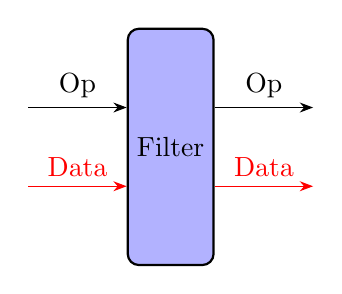
\begin{tikzpicture}
        \begin{pgfonlayer}{stages}
            \node [style=filter_gen, minimum width=1cm, minimum height=3cm] (1) at (0, 0) {Filter};

            %Before
            \draw [style={opChan}] ([yshift=0.5 cm,xshift=-1.25cm]1.west) to["Op"] ([yshift=0.5 cm]1.west);
            \draw [style={daChan}] ([yshift=-0.5 cm,xshift=-1.25cm]1.west) to["Data"] ([yshift=-0.5 cm]1.west);

            %After
            \draw [style={opChan}] ([yshift=0.5 cm]1.east) to["Op"] ([yshift=0.5 cm,xshift=1.25cm]1.east);
            \draw [style={daChan}] ([yshift=-0.5 cm]1.east) to["Data"] ([yshift=-0.5 cm,xshift=1.25cm]1.east);
        \end{pgfonlayer}
        \begin{pgfonlayer}{edgelayer}
        \end{pgfonlayer}
    \end{tikzpicture}
    \column{0.4\textwidth}
    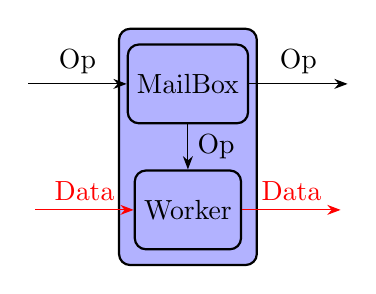
\begin{tikzpicture}
        \begin{pgfonlayer}{stages}
            \node [style=filter_gen, minimum width=1.75cm, minimum height=3cm] (1) at (0, 0) {};
            \node [style=filter_gen, minimum width=1cm, minimum height=1cm] (MailBox) at (0, 0.8) {MailBox};
            \node [style=filter_gen, minimum width=1cm, minimum height=1cm] (Worker) at (0, -0.8) {Worker};

            %Before
            \draw [style={opChan}] ([xshift=-1.25cm]MailBox.west) to["Op"] (MailBox.west);
            \draw [style={daChan}] ([xshift=-1.25cm]Worker.west) to["Data"] (Worker.west);

            % Between
            \draw [style={opChan}] (MailBox.south) to["Op"] (Worker.north);

            %After
            \draw [style={opChan}] (MailBox.east) to["Op"] ([xshift=1.25cm]MailBox.east);
            \draw [style={daChan}] (Worker.east) to["Data"] ([xshift=1.25cm]Worker.east);
        \end{pgfonlayer}
        \begin{pgfonlayer}{edgelayer}
        \end{pgfonlayer}
    \end{tikzpicture}
    \end{columns}
\end{frame}

\begin{frame}{Experimental Study: Decoupled Event Handling (II)}
    We generated instances with different number of operations and measure the execution time of \DPmst\ of different file sizes with and without the MailBox/Worker optimization.

    \begin{table}[H]
        \centering
        \begin{tabular}{@{}lrr@{}}
        \toprule
        Operations & No optimization & With optimization \\ \midrule
        7500       & 1h 9m 31.48s    & 57m 28.23s        \\
        10000      & 3h 46m 46.73s   & 2h 44m 14.19s     \\ \bottomrule
        \end{tabular}
    \end{table}
\end{frame}


\begin{frame}{Experimental Study: Comparison}
    \centering
    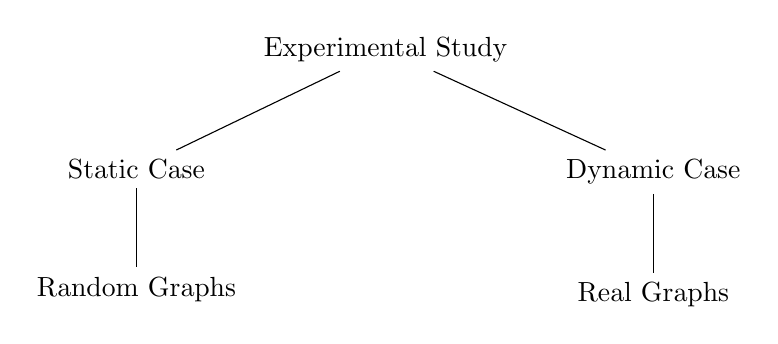
\begin{tikzpicture}
        \node  (0) at (0, 0) {Experimental Study};
        \node [below left=1cm and 0.5cm of 0] (1) {Static Case};
        \node [below right=1cm and 0.5cm of 0] (2) {Dynamic Case};
        \node [below=1cm of 1] (3) {Random Graphs};
        \node [below=1cm of 2] (4) {Real Graphs};
        \draw[style={tree_edge}]{} (0) to (1);
        \draw[style={tree_edge}]{} (0) to (2);
        \draw[style={tree_edge}]{} (1) to (3);
        \draw[style={tree_edge}]{} (2) to (4);
    \end{tikzpicture}
    
    \textcolor{white}{Here goes some text}
    
    \justifying
    We measured elapsed wall-clock time $T(k,n,p)$ and we refer to  absolute speed up and efficiency as: 
    \begin{itemize}
        \item \textit{Absolute speedup}: $speedup_a(k) = T(1, n, p)/T(k, n, p)$.
        \item \textit{Efficiency}: $speedup_a(k)/k$.
    \end{itemize} 

\end{frame}

\begin{frame}{Experimental Study: Static Case (I)}
    20 static binomial random graphs for each combination of:
    \begin{itemize}
        \item Number of vertices: $n \in \{ 10^3, 2\cdot10^3, 10^4, 5\cdot10^4 \}$
        \item Edge probability: $p \in \{ 0.25, 0.50, 0.75, 0.90\}$
    \end{itemize}

\end{frame}

\begin{frame}{Experimental Study: Static Case (II)}
    \begin{figure}
            \centering
            \includegraphics[width=1\linewidth]{figures/SomeDensities_mixed.pdf}
    \end{figure}

    \begin{figure}
            \centering
            \includegraphics[width=1\linewidth]{figures/SpeedUpDPandFK_sample.pdf}
    \end{figure}
\end{frame}

\begin{frame}{Experimental Study: Dynamic case (I)}
We obtained some realistic dynamic graphs collected from a public repository.~\footnote{\href{https://DynGraphLab.github.io/}{\texttt{https://DynGraphLab.github.io/}}}. 

\begin{table}[H]
\centering
\begin{tabular}{@{}llll@{}}
\toprule
Dataset        & Vertices  & Operations & Density \\ \midrule
amazon-ratings & 495,452   & 476,728    & $1.94\cdot10^{-6}$ \\
as-caida       & 31,379    & 19,468     & $1.21\cdot10^{-4}$ \\
frwiki         & 2,212,682 & 31,624,375 & $6.46\cdot10^{-6}$ \\
movielens10m   & 49,847    & 384,585    & $1.55\cdot10^{-4}$ \\
simplewiki     & 100,312   & 889,016    & $8.84\cdot10^{-5}$ \\ \bottomrule
\end{tabular}
\end{table}
\end{frame}

\begin{frame}{Experimental Study: Dynamic case (II)}
    \begin{table}[]
    \centering
    \begin{tabular}{lrrr}
        \toprule
        Dataset            & \FKruskal & \DPmst\   & SpeedUp \\ \midrule
        {\tt as-caida}     &  1h 30min &  1h 19min & 1.14    \\
        {\tt movielens10m} &  1h 39min &  1h 20min & 1.24    \\
        {\tt simplewiki}   & 17h  8min & 11h 29min & 1.48    \\
        \bottomrule
    \end{tabular}
    \end{table}

    \begin{figure}
        \centering
        \includegraphics[width=\textwidth]{figures/RealGraphs.pdf}
    \end{figure}
\end{frame}

\section{Conclusion \& Future Work}
\begin{frame}{Conclusion \& Future Work} \justifying
    \DPmst\ proved to be a highly effective algorithm for computing and maintaining an \mst\ with substantial parallelization, surpassing other algorithms in both performance and scalability. This project validates the \dpm's potential for solving complex graph problems and highlights its broader applicability in parallel computing and provides critical optimizations for the framework itself.
    
    There are many open research directions to explore. For instance:
    \begin{itemize}
        \item Extend the implementation to use several machines
        \item Broader experiments with algorithms for maintaining an \mst\ of dynamic graphs
        \item Explore other data structures inside the filter stage
        \item More precise analysis of cost
        \item ...
    \end{itemize}
\end{frame}


\begin{frame}{Conclusion \& Future Work} \justifying
    A short-paper of this work has been accepted for presentation in the Poster session at the Euro-Par 2024 conference.
\end{frame}


\end{document}